%version of 07-22-20

\chapter{$\oplus$ Pointers to Advanced Topics on Graphs}
\label{ch:advanced-topics}

This chapter introduces four graph-related topics that are typically not covered---at least in depth---early in the curriculum, but that are important enough that the reader should at least be aware of them.  The topics we choose are motivated by studies in virtually every computational area that benefits from graph-theoretic models.  We have tried to present each topic at a level of discourse that will prepare the interested reader to delve more deeply into the material, yet at a level of informality that will make the material accessible to the more casual reader.  We thus strive for an intuitive presentation that will not lead any reader astray.

\smallskip

\begin{itemize}
\item
Section~\ref{sec:graph-decompose} focuses on the myriad computations on graphs that can be accomplished efficiently via recursive algorithms that (1) decompose an input graph $\g$; (2) process the resulting subgraphs of $\g$; (3) reassemble the processed graphs.

\index{graph!graph separators} \index{graph!graph decomposition}

\medskip\item
Section~\ref{sec:graph-evolve}  introduces the increasingly important topic of graphs whose structure changes dynamically over time.  One timely instance of such dynamic evolution is the connectivity graph of the Internet.

\index{graph!evolving graphs} \index{graph models within social media}

\medskip\item
Section~\ref{sec:hypergraphs} introduces {\it hypergraphs}---generalized graphs that allow relationships among {\em multiple} entities/vertices, in contrast to the purely {\em binary} relationships demanded by graphs' {\em two-element} edges.  Hypergraph-based models find application in areas as diverse as:
  \begin{itemize}
  \item
{\it social networks:} Hyperedges describe, e.g., collaboration and collusion.
  \medskip\item
{\it electronic networks:} Hyperedges enable the design of equi-potential vertices in 
voltage-driven technologies such as {\it VLSI}.
  \medskip\item
{\it communication networks:} Hyperedges model bus-oriented communication.
  \end{itemize}

\index{hypergraph} \index{graph!hypergraph} \index{VLSI} \index{bus-oriented communication}

\medskip\item
Section~\ref{sec:multigraphs} introduces {\it multigraphs}---generalized graphs that allow multiple edges between each pair of vertices.  In contrast to other advanced topics, multigraphs are used more {\em internally}, as an algorithmic device, than {\em externally}, as an abstract model of ``real'' structures.  E.g., using multigraphs to replace integer-weighted edges with multiple unweighted edges with the same endpoints can trigger algorithmic ideas.

\index{graph!multigraphs} \index{multigraphs}
\end{itemize}

\section{Graph Decomposition}
\label{sec:graph-decompose}
\index{graph!decomposition}
\index{graph!bisector}
\index{graph!separator}

\noindent \fbox{\begin{minipage}{0.96\textwidth}
{\bf Topic-specific references}

\smallskip

F.~Annexstein, M.~Baumslag, A.L.~Rosenberg (1990): Group action graphs and parallel architectures.  {\it SIAM J.~Comput.~19}, 544--569.

\smallskip

C.E.~Leiserson (1985): Fat-trees: Universal networks for hardware-efficient supercomputing.
{\it IEEE Trans.~on Computers, C-34}(10), 892--201.

\smallskip

R.J.~Lipton, R.E.~Tarjan (1979): A separator theorem for planar graphs.  {\it SIAM J.~Applied Mathematics 36}(2), 177--189.

\smallskip

A.L.~Rosenberg and L.S.~Heath (2001): {\it Graph Separators, with Applications}.  Kluwer Academic/Plenum Publishers, New York.

\smallskip

J.D.~Ullman (1984): {\it Computational Aspects of VLSI.}. Computer Science Press, Rockville, Md.

\end{minipage}
}

\bigskip

\noindent
The reader will certainly have noted that some ``named'' graphs are, intuitively, more tightly interconnected than others---with the cycle and clique being the antipodal examples.  Even from a purely intellectual vantage point---and all the more so from an algorithmic vantage point---it would be of interest to be able to quantify the tightness of a graph's interconnectedness.  Among  the various measures that have been proposed for this task, one stands out for its myriad algorithmic implications: the notion of {\it graph separator}.  In fact, this notion appears in the literature in several flavors.  An $n$-vertex, $e$-edge graph $\g$ has:
\begin{itemize}
\item
an {\it $\alpha$-edge separator} of size $k$---where $\alpha$ is a real number with $\alpha \leq 1/2$  and $k$ is an integer with $k < n$---precisely if:

\index{graph!$\alpha$-edge separator of size $k$}

\smallskip

one can partition $\g$ into two disjoint (not-necessarily connected) subgraphs, each having 
$\leq \alpha n$ vertices, by removing $\leq k$ edges from $\g$.

\medskip\item
a {\it $\alpha$-vertex separator} of size $\ell$, where $\alpha$ is a real number with  $\alpha \leq 1/2$ and $\ell$ is an integer with $k < e$, precisely if:

\index{graph!$\alpha$-vertex separator of size $\ell$}

\smallskip

one can partition $\g$ into two disjoint (not-necessarily connected) subgraphs, each having
$\leq \alpha n$ vertices, by removing $\leq \ell$ vertices from $\g$.
\end{itemize}
We replace the term ``separator'' with the term {\em ``bisector''} if both subgraphs after a separation operation have $\leq \left\lceil \frac{1}{2} n \right\rceil$ vertices.

\index{graph!edge bisector} \index{graph!vertex bisector}

\medskip

Commonalities and differences in graphs' inherent separator sizes are often not visually obvious.  For illustration, referring to the ``named'' graphs of Section~\ref{sec:graphs-important-families}:
\begin{itemize}
\item
It is certainly obvious that cycles are easier to bisect than cliques, as measured by either edge or vertex bisectors.
\medskip\item
It is far less clear that de Bruijn networks and hypercubes are roughly equal in ease of bisection, as measured by vertex bisectors.
\end{itemize}

\smallskip

Similarity in separation behavior often has very important algorithmic consequences.  For instance, the closeness in separation characteristics between de Bruijn networks and hypercubes manifests itself in a large range of algorithmic applications.  The range of such applications is hinted at by sources that study the algorithmics of laying out VLSI circuits (cf., [Leiserson, 1985]) and sources that study the ability of a network's interconnections to host a range of communication patterns that enable efficient parallel computation and communication (cf., [ Annexstein, Baumslag, Rosenberg, 1990], [Leiserson, 1985], and [Ullman, 1984].

\medskip

There is a large literature that develops the algorithmics of finding small separators for computationally significant families of graphs.  An early star in the firmament of such studies is the discovery in [Lipton, Tarjan, 1979] of a $1/3$-vertex separator of size $\sqrt{8n}$ for $n$-vertex planar graphs.  The dual problem of finding lower bounds on the sizes of graph separators is a bit sparser but, of course, no less significant.  The reader can find a comprehensive exposition of the theory of graph separators in [Rosenberg, Heath, 2001], including both the mathematics that yields lower bounds on separator sizes and the algorithmics that yields upper bounds.


\section{Graphs Having Evolving Structure}
\label{sec:graph-evolve}
\index{graph!with evolving structure}

\noindent \fbox{\begin{minipage}{0.96\textwidth}
{\bf Topic-specific references}

\smallskip

W.~Aiello, F.R.K.~Chung, L.~Lu (2000): A random graph model for massive graphs.  {\it 32nd Ann.~Symp.~on the Theory of Computing}.

\smallskip

A.L.~Barab\'{a}si, R.~Albert (1999): Emergence of scaling in random networks.  {\it Science (286)}, 509--512.

\smallskip

B.~Bollobas (1985): {\it Random Graphs}.  Academic Press, N.Y.

\smallskip

T.~Bu, D.~Towsley (2002): On distinguishing between internet power-law generators.  {\it IEEE INFOCOM'02}.

\smallskip

Q.~Chen, H.~Chang, R.~Govindan, S.~Jamin, S.~Shenker, W.~Willinger (2002):
The origin of power laws in internet topologies revisited.  {\it IEEE INFOCOM'02}.

\smallskip

M.~Faloutsos, P.~Faloutsos, C.~Faloutsos (1999): On power-law relationships of the internet topology.  {\it ACM SIGCOMM'99}.

\smallskip

S.~Jaiswal, A.L.~Rosenberg, D.~Towsley (2004): Comparing the structure of power-law graphs and the Internet AS graph.  {\it 12th IEEE Int'l Conf.~on Network Protocols (ICNP'04)}.

\smallskip

H.~Tangmunarunkit, R.~Govindan, S.~Jamin, S.~Shenker, W.~Willinger (2002):
Network topology generators: Degree-based vs. structural.  {\it ACM SIGCOMM'02}.

\smallskip

E.~Zegura, K.L.~Calvert, M.J.~Donohoo (1997): A quantitative comparison of graph-based models for internetworks.  {\it IEEE/ACM Trans.~on Networking, 5}(6), 770--783.
\end{minipage}
}

\bigskip

A large variety of problems in the area of graph algorithms involve graphs---especially 
trees---whose structures evolve over time.  Such evolution is observed, e.g., in the study of ``classical" algorithmic problems such as {\it Minimum Spanning Tree} and {\it Branch and Bound}; see, e.g., \cite{CLRS}.  What is certain to be more exciting to the reader, though, are the ``modern'' topics where one encounters graphs with evolving structure, such as {\it social networks} and {\it inter-networks} (e.g., {\it IoT},  the {\it Internet of Things}).

\medskip

For ``classical'' topics, such as the two we have mentioned, the material in Chapters~\ref{ch:Graphs1} and~\ref{ch:Graphs2} will provide the reader with the background necessary to deal with graph evolution.  Indeed, evolution emerges as an inevitable concomitant of the algorithmics that is superimposed upon the traditional structures of graph theory.  The challenge of evolution is to assimilate new algorithmics, not new mathematics.

\medskip

\index{graph!with evolving structure!social networks}
\index{graph!with evolving structure!inter-networks}

In contrast, the ``modern'' topics we have mentioned do require the assimilation of new 
mathematics.  Dealing successfully with the algorithmic issues that arise with social networks and inter-networks requires the reader to understand the structures of the evolving graph-oriented systems and how evolution changes these structures.  Among the interesting (and valuable) mathematical questions that one can pose is: If you are a new vertex ``applying" to join an evolving network, which vertex in the network is the best one to connect to, in order to best facilitate your interactions or influence within the community.  The latter topic leads, e.g., to the study of {\em power-law} networks.

\index{graph!with evolving structure!social networks!power-law networks}
\index{graph!with power-law degree growth patterns}

\bigskip

\noindent \fbox{
\begin{minipage}{0.96\textwidth}
{\bf Explanatory note}.

\smallskip

An evolving network {\it obeys a power law} if there exists a real number $\gamma >0$ with the following property.  For all network vertices having sufficiently large vertex-degrees, the fraction of vertices that have degree $k$ is proportional to $k^{-\gamma}$.
\end{minipage}
}
\bigskip

Little of the abstract work on power-law networks would likely be studied in depth in an early course; indeed, the structure of these networks is not yet well understood even in advanced settings.  Attempts to understand power laws with rigor have led to a number of competing, rather sophisticated, abstract models---see, e.g.,  [Aiello, Chung, Lu, 2000], [Barab\'{a}si, Albert, 1999], [Bollobas, 1985], and [Chen, Chang, Govindan, Jamin, Shenker, Willinger, 2002]---and numerous studies have attempted to understand when the abstract models reflect reality more or less faithfully---see, e.g.,
[Bu, Towsley, 2002], [Faloutsos, Faloutsos, Faloutsos, 1999], [Jaiswal, Rosenberg, Towsley, 2004] [Tangmunarunkit, Govindan, Jamin, Shenker, Willinger, 2002], and [Zegura, Calvert, Donohoo, 1997].

\bigskip

\noindent \fbox{\begin{minipage}{0.96\textwidth}
{\bf Explanatory note}.

\smallskip

We have just cited several sources that deal with the evolving formal notion of power-law graph.  This apparent overkill---wouldn't one citation suffice?---is intentional.
\end{minipage}
}

\smallskip

\noindent \fbox{\begin{minipage}{0.96\textwidth}
{\bf Explanatory note} (cont'd).

\smallskip

We have just cited several sources that deal with the evolving formal notion of power-law graph.  This apparent overkill---wouldn't one citation suffice?---is intentional.
As new ``real-life" concepts emerge which need mathematical modeling---in this case, as the social media become an object of increasing study---there is inevitably a period in which competing mathematical models are proposed.  All of the models that have emerged thus far capture the central feature of power laws.  But every mathematical model embodies ``side" features that go beyond the targeted central feature.  We must allow multiple models to coexist until we have the opportunity to compare all of the models' side features.  Only after this vetting period will the scientific community converge on a single mathematical model of a ``real-life" concept such as ``power-law graph".
\end{minipage}
}


\section{Hypergraphs}
\label{sec:hypergraphs}
\index{graph!generalization to hypergraphs} \index{hypergraph}

\noindent \fbox{\begin{minipage}{0.96\textwidth}
{\bf Topic-specific references}

\smallskip

F.~Amato, F.~di Lillo, V.~Moscato, A.~Picariello, G.~Sperl (2017): Influence analysis in online social networks using hypergraphs.  {\it IEEE Int'l Conf.~on Information Reuse and Integration}.

\smallskip

D.~Liu, N.~Blenn, P.~Van Mieghem (2010): Modeling social networks with overlapping communities using hypergraphs and their line graphs.  Report arXiv:1012.2774, Dec.~2010, {\tt http://cds.cern.ch/record/1314107}.

\smallskip

L.~Lov\'{a}sz (1973): Coverings and colorings of hypergraphs.  {\it 4th Southeast Conf.~on Combinatorics, Graph Theory, and Computing}, 3--12.

%\smallskip
%C.~Mead and L.~Conway (1979): {\it Introduction to VLSI Systems}.  Addison-Wesley, Reading, MA., (ISBN 0201043580).

\smallskip

A.L.~Rosenberg (1985): A hypergraph model for fault-tolerant VLSI processor arrays.  {\it IEEE Trans.~Comput.~C-34}, 578--584.

\smallskip

A.L.~Rosenberg (1989): Interval hypergraphs.  In {\it Graphs and Algorithms} (R.B.~Richter, ed.) {\it Contemporary Mathematics 89}, Amer.~Math.~Soc., 27--44.
\end{minipage}
}

\bigskip

\noindent
A large variety of modern computing-related topics benefit from the structure inherent in graph-theoretic models but do not comfortably conform to the {\em binary} relationships imposed by graphs' having {\em two} vertices per edge.  We now discuss a model that retains the general structure of graph-theoretic models while it abandons the {\em binary} constraint in edge-membership---this is the {\em hypergraph} model.  A hypergraph has vertices that play exactly the same role as with graphs, but in place of a graph's $2$-element edges, a hypergraph has {\em hyperedges}, each being a set of vertices whose size is not restricted to $2$.  A rather general treatment of hypergraphs can be found in the comprehensive graph-theory text \cite{Berge73}; a specialized article that focuses on hypergraph-related versions of several topics from Chapters~\ref{ch:Graphs1} and~\ref{ch:Graphs2}, including vertex-coloring, is [Lov\'{a}sz, 1973].

\smallskip

Because of their inherent conceptual complexity, hypergraphs as graph-theoretic objects are usually relegated to advanced courses.  However, the literature contains many studies of hypergraphs that are ``fine-tuned'' for specific computing-related applications.  Several of these studies should be accessible without extensive mathematical background.  Sample  computing-related applications that benefit from hypergraph-oriented models include the following.
\begin{itemize}
\item
Bus-connected parallel communication has been part of digital-computer design since its earliest days.  The informal picture of such a system is that there are communication channels which multiple agents can retrieve messages from and post messages to.  In hypergraph-oriented terms: the vertices/communicating agents aggregate into groups/hyperedges.  Each group's agents share ``read/write'' access to a specific channel.  A specialized genre of hypergraph which was invented to study the described scenario is the {\it interval hypergraph} model developed in [Rosenberg, 1989].
\index{hypergraph!modeling bus-connected communication}
\index{hypergraph!interval hyergraph}

\medskip
\item
Modern electronic circuits are implemented using integrated circuit technology, specifically, {\em VLSI: Very Large Scale Integrated circuitry}; the often-informal book \cite{Mead-Conway} provides an introduction to VLSI for the non-specialist.  VLSI technologies are often {\em voltage}-driven, rather than {\em current}-driven.  Accordingly, much of the attention when designing VLSI circuits centers on the coordination of equi-potential points in an electrical  network, rather than on point-to-point transmission of signals.  Hypergraphs are tailor-made for such technologies.

A crucially important issue that arises because of the design strengths and weaknesses of VLSI 
technology is {\it fault tolerance}---how to cope with the inevitable faulty transistors in massive VLSI systems.  A variety of quite-accessible mathematical ideas can provide provocative ideas about this important topic; see, e.g., [Rosenberg, 1985].

\index{hypergraph!modeling integrated circuits} \index{VLSI}

\medskip
\item
Social networks have become so prevalent in society that no one will be surprised to learn that many approaches to modeling the networks' interconnectivity have been studied.  In
Section~\ref{sec:graph-evolve}, we discussed an interconnectivity model based on evolving graphs and clustering within such graphs.  More recently, hypergraph-based models have also been proposed; see, e.g., [Amato, di Lillo, Moscato, Picariello, Sperl, 2017] and [Liu, Blenn, Van Mieghem, 2010].
\index{hypergraph!modeling interconnectivity in social networks}
\end{itemize}

\section{Multigraphs and the Chinese Postman Problem}
\label{sec:multigraphs}
\index{graph!multigraph} \index{multigraph} \index{multiedge}

A {\it multigraph} is a graph-like structure that admits a {\em multiset} of edges, rather than a set.  In detail, a multigraph $\h$ has a set $\n_{\fh}$ of vertices and a {\em multiset} of edges, each edge being a $2$-element set of vertices.  Viewed differently, but equivalently, a pair of vertices in a multigraph can be connected by more than one edge.  Fig.~\ref{fig:EulerianFinal} depicts a ten-vertex multigraph $\h$.
\begin{figure}[hbt]
\begin{center}
       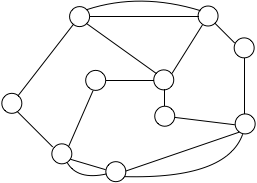
\includegraphics[scale=0.4]{FiguresGraph/EulerienFinal}
       \caption{A $10$-vertex multigraph $\g$ with $3$ multi-edges.}
              \label{fig:EulerianFinal}
\end{center}
\end{figure}
Ten pairs of $\g$'s vertices are connected by single edges; three pairs of $\g$'s vertices are connected by multiedges, each of which (coincidentally) consists of two edges.

\smallskip

We noted earlier that multigraphs were usually an algorithmic tool rather than a modeling tool.  We now present a sample algorithmic use of multigraphs which allows us to extend the concept of Eulerian tour to a family of graphs that lie outside the domain delimited by Proposition~\ref{thm:eulerian-cycle}.  Recall that the proposition asserts that a {\em graph} admits a tour that crosses each edge precisely once if, and only if, each of its vertices has even degree.

\bigskip

From an applied vantage point, {\em pragmatism is often preferable to purity!}  Imagine that one does not have access to an efficient solution for the ``pure'' version of a practically important problem, because some essential precondition is violated.  One is often willing to ``bend the rules" if such ``distortion" will give one access to an efficient solution to the resulting ``not-quite-pure'' version of the problem. 

\medskip

The preceding highlighted dictum can be illustrated via the Euler-tour problem.

\begin{prop}
If a {\em connected} graph $\g$ has an {\em even number of odd-degree vertices}, then we can transform $\g$ to a {\em multigraph} $\g^+$ that admits a tour which crosses every edge precisely once.
\end{prop}

In fact, we can solve this ``distorted" version of the Euler-tour problem in a manner that is algorithmically efficient in the following senses.
\begin{itemize}
\item
{\em The newly added edges preserve the neighbor relation of $\g$.}

\smallskip

As we add the edges that convert $\g$'s edge-set to an edge-{\em multiset}, we never create new adjacencies: Every new edge that we add connects vertices that were already adjacent in $\g$.

\medskip\item
{\em The algorithm adds the fewest number of new edges possible in order to achieve the described tour.}

\smallskip

Say that the multigraph $\g'$ is produced by adding edges to $\g$.  If $\g'$ has fewer edges than $\g^+$, then $\g'$ does {\em not} admit a tour that crosses each edge precisely once.

\medskip\item
{\em The algorithm is computationally efficient: it operates in time polynomial in the size of the graph $\g$.}
\end{itemize}

\medskip

\index{Route Inspection Problem} \index{Chinese Postman Problem} \index{Kwan Mei-Ko}

Our ``distorted" version of the Euler-tour problem is actually a well-known combinatorial optimization problem which is known either as the {\it Route Inspection Problem} or as the {\it Chinese Postman Problem}---the latter name in honor of the Chinese mathematician Kwan Mei-Ko who invented the problem.\footnote{M.-K.~Kwan (1960): Graphic programming using odd or even points.  {\it Acta Mathematica Sinica, 10} (in Chinese), 263--266.  Translated into English in {\it Chinese Mathematics 1} (1962) 273--277.}  These colorful names arise from stories about a person---either a route inspector or a postal employee---who must traverse all of the roads in a village and who wants to avoid extraneous road traversals.

\medskip

We illustrate the problem and an algorithm that solves it.

\smallskip

Fig.~\ref{fig:EulerianInitial} presents a $10$-vertex input $\g$ to our ``distorted" Euler-tour problem. 
\begin{figure}[hbt]
\begin{center}
       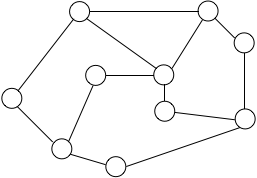
\includegraphics[scale=0.35]{FiguresGraph/EulerienInitial}
       \caption{A $10$-vertex graph which is not Eulerian.}
              \label{fig:EulerianInitial}
\end{center}
\end{figure}
Note that $\g$ is not Eulerian because it has four odd-degree vertices---happily, an even number!  $\g$'s odd-degree vertices are highlighted in Fig.~\ref{fig:EulerianVodd}.
\begin{figure}[hbt]
\begin{center}
       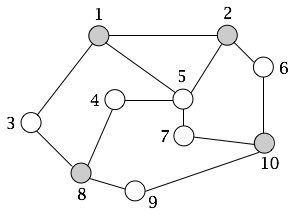
\includegraphics[scale=0.35]{FiguresGraph/EulerianVodd}
       \caption{$\g$ with its $4$ odd-degree vertices highlighted by shading.}
              \label{fig:EulerianVodd}
\end{center}
\end{figure}

\smallskip

We sketch a process that adds a minimally many edges to $\g$ while converting $\g$ to a multigraph that admits a ``distorted" Euler tour. 

\medskip

\noindent {\bf Procedure} {\sf Edge Augmentation}($\g$) \\
/*Construct a shape-inspired pairing function (PF) $\a$*/  \\
{\bf begin}
\begin{description}
\item[Step 1.]
%
Record, for each pair of vertices $u, v \in \n_{\fg}$, the length $\ell(u,v)$ of a {\em shortest path} between $u$ and $v$.  (Recall that $\g$ is connected.)

\smallskip

Computing each length $\ell(u,v)$, together with a length-$\ell(u,v)$ path between $u$ and $v$, can be accomplished in low-degree polynomial time; see \cite{CLRS}.

\medskip\item[Step 2.]
%
Say that $\g$ has $m$ odd-degree vertices $w_1, \ldots, w_m$ ($m=4$ in our illustration).  Create a copy of the $m$-clique $\k_m$ on these $m$ vertices.

\medskip\item[Step 3.]
%
Label each edge $\{u,v\}$ of the clique $\k_m$ with the path-length $\ell(u,v)$.

\medskip\item[Step 4.]
%
Compute a perfect matching of minimal weight in the edge-weighted clique $\k_m$.

\smallskip

Computing minimal-weight perfect matchings can be accomplished in low-degree polynomial time; see \cite{CLRS}.

\smallskip

Fig.~\ref{fig:Eulerianperfectmatching} illustrates the results of this process on our sample graph $\g$.   {\em Note}: The double-edges that we add make the degrees of all odd-degree vertices even.  The double-edge at the top of $\g$ in the drawing makes the degrees of both top vertices even; the length-$2$ double-edge at the bottom of $\g$ in the drawing makes the degrees of both bottom odd-degree vertices even.
\begin{figure}[hbt]
\begin{center}
       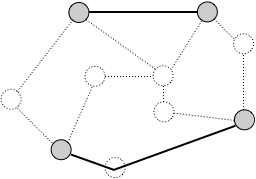
\includegraphics[scale=0.35]{FiguresGraph/EulerienPerfectMatching}
       \caption{A minimum weight perfect matching labelled by the shortest-distances $\ell(u,v)$.}
              \label{fig:Eulerianperfectmatching}
\end{center}
\end{figure}

\medskip\item[Step 5.]
%
Replace each weighted edge produced by the process by an appropriate number of multi-edges.

\smallskip

Fig.~\ref{fig:EulerianFinal} performs this last step for the weighted graph of Fig.~\ref{fig:Eulerianperfectmatching}.
\end{description}
{\bf end} {\sf Edge Augmentation}

\bigskip

Our augmented multigraph $\g^+$ now has all even vertex-degrees.  We can, therefore, adapt the Euler-tour algorithm from the proof of Proposition~\ref{thm:eulerian-cycle}(a) to produce a tour of $\g^+$ that crosses each multiedge precisely once.  The required adaptation simply views distinct multiedges as distinct edges for the purposes of the mandate to ``leave a vertex by a different edge than you entered on".

\medskip

The importance of the notion of multigraph in this story is that it gave us a perspicuous bridge between the strongly algorithmic world of edge-weighted graphs and the purely graph-theoretic world that underlies Proposition~\ref{thm:eulerian-cycle}.  This can be a valuable bridge when computing with graph-theoretic models.
